\section{Compressed Sensing Image Reconstruction for MeerKAT} \label{intro}
Image reconstruction problems arise in a variety of fields. From Medicine to Astronomy, imaging instruments are dealing with some level of corrupted measurements. Noise from the instrument itself, external interference or loss of samples, all introduce corruptions that a reconstruction algorithm should remove. 

An algorithm should decide which part of the image is noise, and which is the image. It needs a prior for what an image is. This has led to the theory of Compressed Sensing\cite{candes2006robust, donoho2006compressed}, which gives us a theoretical framework for analysis and design of reconstruction algorithms. It gives us theoretical guarantees that, under the right prior, an algorithm is guaranteed to reconstruct the observed image, potentially  above the accuracy limit of the instrument.

In this work we apply the theory of Compressed Sensing to the reconstruction problem of Radio Interferometers. More specifically, we apply it on the MeerKAT interferometer, which poses the problem on a new scale of data volume. The raw measurement easily take up several hundreds of gigabytes, which should get reconstructed to an image. The current state of the art reconstruction is based on the CLEAN\cite{rich2008multi, rau2011multi} algorithm. Although newer Compressed Sensing reconstructions showed superior image quality\cite{girard2015sparse, dabbech2018cygnus}, they are more expensive to compute than CLEAN.

MeerKAT in the future will only produce more data. The reconstruction algorithm has to be scalable and sooner or later distributable. So far, state of the art CLEAN algorithm can distribute some steps, has limited capabilitiy of distribution. How to get a reconstruction algorithm to scale for future MeerKAT data is still an open problem.

In this project we investigated different reconstruction architectures for Compressed Sensing. Our task was to reduce the overall runtime costs compared to CLEAN. We created a Compressed Sensing reconstruction in a new architecture, which uses the direct Fourier Transform. It scales with the number of sparse components. We showed superior reconstruction quality than CLEAN.  We extrapolate the runtime costs of our approach on MeerKAT scale reconstructions. Sadly, this architecture alone does not lead to runtime cost reduction compared to CLEAN or other state of the art approaches.

Nevertheless, it our algorithm might be easier to distribute. When combined with other concepts, we might arrive at a cheaper reconstruction algorithms.

We postulate that there is no single step which will get us to to the target of a highly scalable, highly distributable Compressed Sensing reconstruction. At the current point, there is no obvious way

We begin by introducing the basic image reconstruction problem in radio interferometry and show what the current architecture of interferometric reconstruction algorithms, the Major Cycle. Section \ref{meerkat} introduces the difficulties of imaging MeerKAT data. We  move towards competing architectures in section \ref{killmajor}. In the following sections \ref{cd}, \ref{results} and \ref{scale} we introduce our Compressed Sensing Reconstruction, show the reconstruction quality on simulated MeerKAT data and extrapolate the runtime costs on a real world MeerKAT measurement.

\subsection{The basic reconstruction problem in Radio Interferometry}\label{intro:basic}
Real world radio interferometers have complicated measurement equations. They become even more complicated for large interferometers like MeerKAT. These problems get addressed in section \ref{meerkat}. This section looks at the basic measurement equation of a radio interferometer \eqref{intro:measurement} and discusses the two fundamental challenges for radio interferometry image reconstruction. 

\begin{equation}\label{intro:measurement}
V(u, v) = \int\int I(x, y) e^{2 \pi i (ux+vy)} \: dx \: dy
\end{equation}

\begin{equation}\label{intro:cs}
\underset{x}{minimize} \: \left \| V - Fx \right \|_2^2 + \lambda \left \| x \right \|_1
\end{equation}



An interferometer measures Fourier Components $V$ (called Visibilities in Radio Astronomy) from the sky image $I$ at position $x$ and $y$. The term $e^{2 \pi i (ux+vy)}$ represents the two dimensional Fourier Transform. The task is to reconstruct the observed image $I$ from the measured Visibilities $V$. In theory this task is trivial: Since the inverse Fourier Transform exists, we can reconstruct the image $I$ by calculating the inverse Fourier Transform of $V$. However, two properties of the Visibilities make this task challenging in practice:

\begin{enumerate}
	\item Non-uniform sampling pattern in Visibility space
	\item Incomplete Visibility coverage. 
\end{enumerate} 

\textit{Property 1:} We want to reconstruct an image with uniformly spaced pixels. The instrument defines the sampling pattern in Visibility space and does not correspond to the exact pixels of the reconstructed image. This property keeps us from using the Fast Fourier Transform. The naive inverse Fourier Transform can still be calculated, but it has a quadratic runtime and does not scale to the data volume of interferometers. Current reconstruction algorithms use the non-uniform Fast Fourier Transform. The non-uniform FFT approximates the non-uniform Fourier Transform. 

\textit{Property 2:} Interferometers sample only a limited set of Visibilities. It does not have all information for reconstruction. When the inverse Fourier Transform is applied on the Visibilities, the resulting image is corrupted by the incomplete Visibilities. It contains structures which where introduced by the interferometer and were not observed. With only knowing the incomplete set of Visibilities a reconstruction algorithm has to decide which image structures were truly measured, and which are due to the instrument. This forms an ill-posed inverse problem. There are many images that fit the measurements, and a small change in the Visibilities can lead to a very different reconstruction. 

CLEAN represents the instrumental effect with a Point Spread Function (PSF). After the non-uniform FFT produced the 'dirty' image, CLEAN tries to reconstruct observed image with a deconvolving the 'dirty' image with the PSF. Note however that both CLEAN nor the non-uniform FFT are approximations. In real world reconstructions, these two approximations are used in the major cycle architecture to increase the reconstruction accuracy. 

%The CLEAN algorithms approximate the observed image with a deconvolution: The inverse Fourier Transform produces a corrupted image. The observed image was convolved with a known Point Spread Function (PSF), which represents the instrument corruption. Finding a deconvolution reconstructs the observed image. The deconvolution is still an ill-posed problem, there are potentially many possible deconvolutions, and a small change in the input can lead to a very different output. Furthermore the CLEAN algorithms produce a greedy approximation of the deconvolution. 


\subsection{The Major Cycle Architecture}
Major cycle was created with CLEAN in mind. Compressed sensing reconstructions use essentially the same architecture with minor modifications. 

\begin{equation}\label{intro:clean}
\underset{x}{minimize} \: \left \|  I_{Dirty} - x \star PSF \right \|_2^2 + \lambda \left \| x \right \|_1 \quad, \quad I_{Dirty} = \hat{F}^{-1} V
\end{equation}

%sparsity in the image domain.


A CLEAN image reconstruction for radio interferometers consists of two different steps: A non-uniform FFT, which approximates the inverse Fourier Transform efficiently and an deconvolution algorithm, which approximates the instrumental effects on the image (typically based on CLEAN). These two approximations are an error source of the reconstruction. The major cycle architecture \ref{intro:major} therefore tries to iteratively minimize the errors of the non-uniform FFT and the deconvolution over several iterations.

\begin{wrapfigure}{r}{0.6\textwidth}
	\centering
	\vspace{-10pt}
	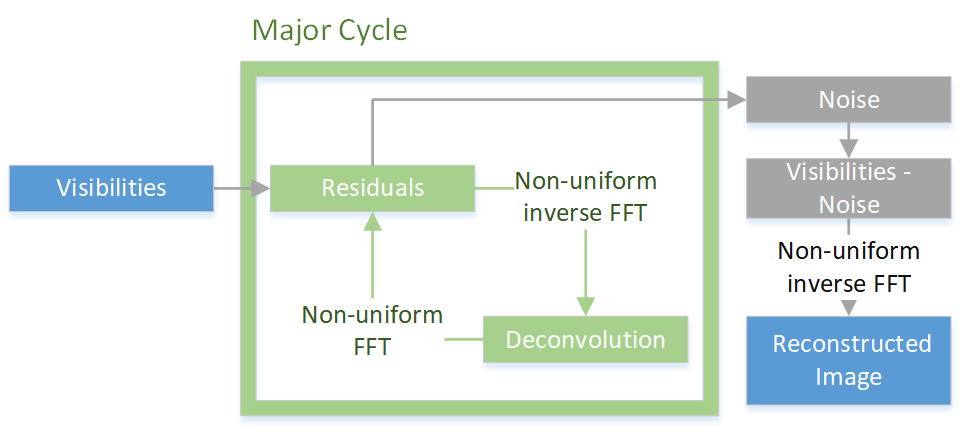
\includegraphics[width=1.0\linewidth]{./chapters/01.intro/Major-Minor.png}
	\caption{The Major Cycle Framework}
	\label{intro:major}
	\vspace{-10pt}
\end{wrapfigure}

The first major cycle uses the non-uniform inverse FFT to approximate the 'dirty' image from the Visibilities. The deconvolution algorithm decides parts which parts belong to the observed image and which are due to instrumental and other noise effects. It returns the noise part of the image, which gets transformed back into residual Visibilities. The next major cycle iteration continues with the residual Visibilities. The residual Visibilities get minimized until they contain only the instrumental effects and noise.

After several major cycles the residual  on a regularly spaced image which has a small error from non-uniform samples, and a small error from incomplete measurements.

Compressed sensing reconstructions essentially use the same architecture, although with minor alterations. In general, they keep a similar scheme of forward/backward non-uniform FFT, but do not use a deconvolution in image pace. Instead, they analyse constraints defined on the image (For example all pixels should be non-negative), and try to find the Visibilities that minimize the constraint violations.

For CLEAN reconstructions, the forward/backward non-uniform FFT are the most expensive operations, while the deconvolution is negligible. The compressed sensing algorithms tend to require more major cycle iterations to converge and the image constraint analysis tends to be more expensive than CLEAN deconvolutions. Current research into compressed sensing reconstructions is focussed on reducing the number of major cycles\cite{dabbech2018cygnus}. 

%Different architecture, but has to somehow handle all the difficulties that arise from imaging meerkat data.


%compressed sensing got rid of the miinor cycle, but essentially kept the major cycle framework
%have to handle own problems in a new architecture






